Laser cooling for the \ce{^9Be+} ion is done with a Toptica TA-FHG Pro tuned to 313 nm with a peak power of 400 mW. The laser is detuned by 400 MHz from the \ce{^2S1/2} to \ce{^2P3/2} transition. We let the light

\begin{figure}[H]
	\centering
	\missingfigure{Be electronic structure}
	\caption{Electronic structure of \ce{^9Be+}. Laser cooling is done with 313 nm light tuned from the \ce{^2S1/2} to \ce{^2P3/2} state.}
\end{figure}

The scatter rate of two level system is defined as:

\begin{equation}
	\rho_{pp} = \frac{a}{2} \frac{s}{a+s+4(\delta/\Gamma)^2}
\end{equation}

\begin{equation}
	f_L = \frac{a \Gamma}{\Delta^2 + \Gamma^2/4}
\end{equation}

\begin{equation}
	I_s = \frac{\pi h c}{3 \lambda^3 \tau}
\end{equation}

\begin{equation}
	s_0 = \frac{I}{I_s}
\end{equation}

Where $\rho_{pp}$ is the fraction of the population in the excited P-state, $s$ is the saturation parameter, $\Gamma$ is the transition linewidth, $\delta$ is the detuning from resonance, and $a$ is an overall scaling parameter encompassing all of the efficiencies associated with the optical collection and detection.


Ideally, having a single ion in the trap while sweeping the frequency or power would allow us to determine the saturation parameter, and thus the fraction of \ce{Be+} in the excited \ce{^2P3/2} state. Due to the size and depth of our ion trap, we cannot reliably load only one ion. On top of that, the most common residual gasses in a vacuum chamber, \ce{H2O} and \ce{H2} both readily react with \ce{Be+} in the excited state. The pressures we reach, indicate that we may expect reaction rates of order once per 10 seconds.

\begin{figure}[H]
	\centering
	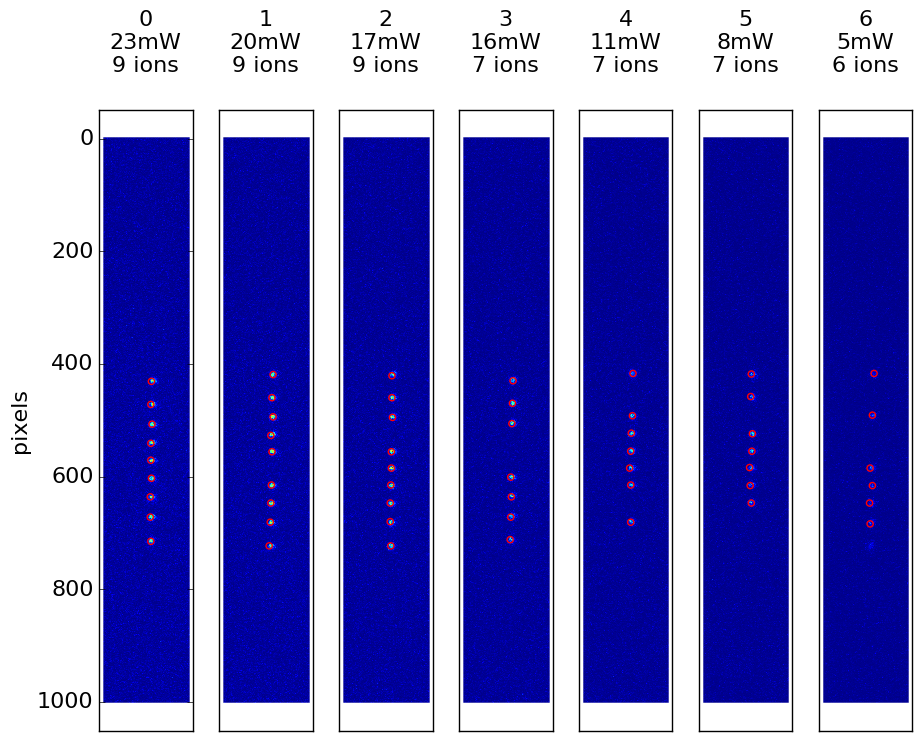
\includegraphics[width=0.8\textwidth]{images/ion_images.png}
	\caption{Set of ion images taken at various 313 nm powers with an algorithm that identifies individual ions}
	\label{fig: ion image set}
\end{figure}

\newpage
\begin{figure}[H]
	\centering
	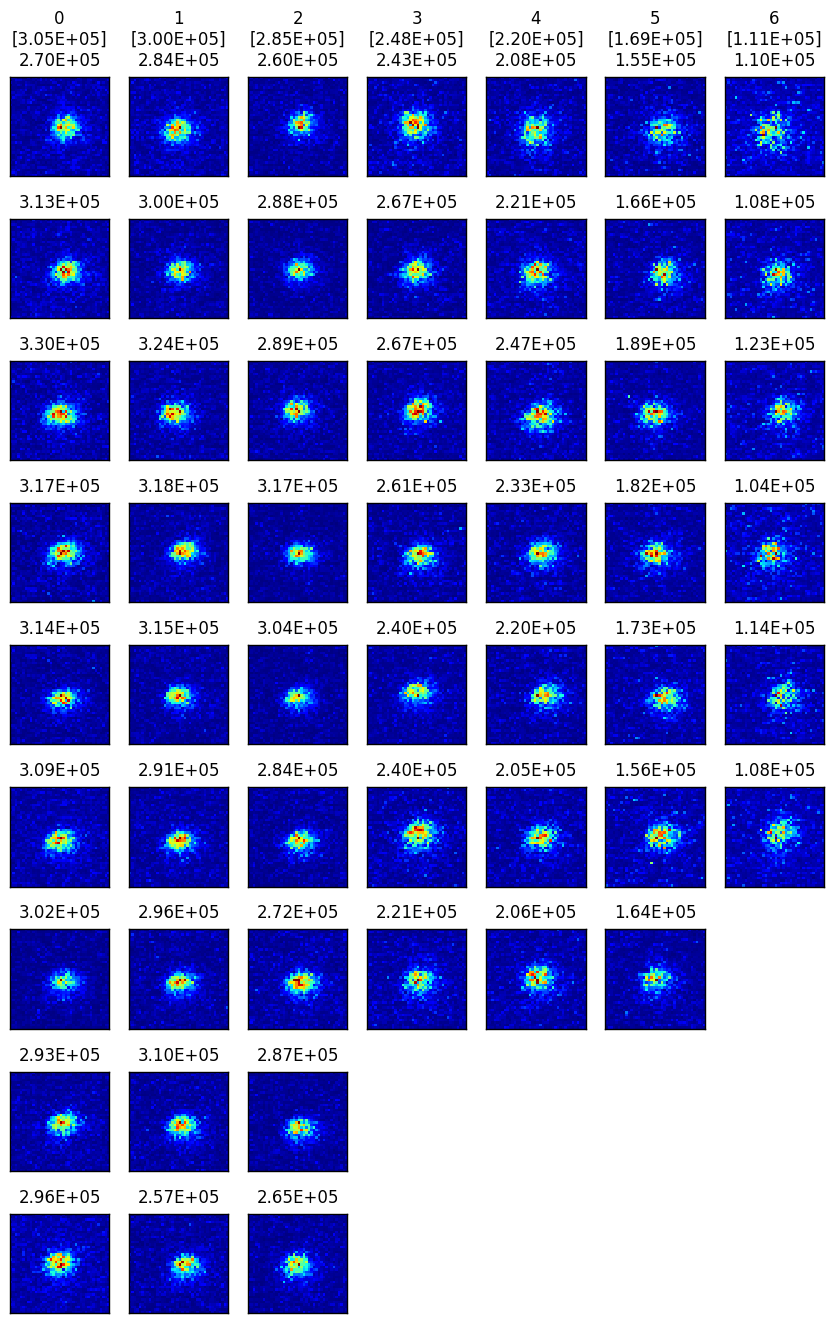
\includegraphics[height=0.7\paperheight]{images/isolated_ions.png}
	\caption{Individual ions identified from images in figure \ref{fig: ion image set}. Integrated fluorescence counts shown for each image as well as averaged value in brackets.}
\end{figure}

\begin{figure}[H]
	\centering
	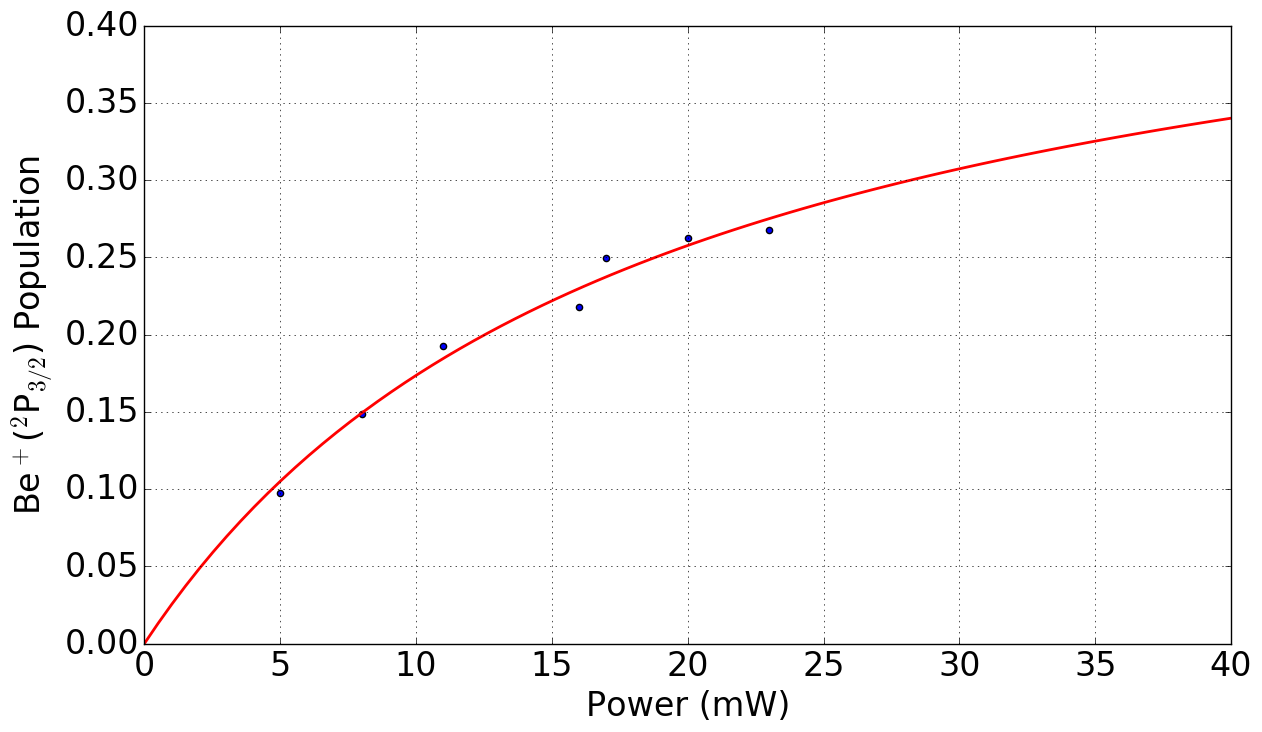
\includegraphics[width=0.8\textwidth]{images/P_state_curve.png}
	\caption{P-state fraction curve fitted to incident laser power at a fixed detuning of $\omega_l = \omega_0 - \Gamma/2$.}
\end{figure}